\documentclass[a4paper]{article}
\usepackage[utf8]{inputenc}
\usepackage[russian]{babel}
\usepackage[T2]{fontenc}
\usepackage[warn]{mathtext}
\usepackage{graphicx}
\usepackage{amsmath}
\usepackage{floatflt}
\usepackage[left=20mm, top=20mm, right=20mm, bottom=20mm, footskip=10mm]{geometry}


\graphicspath{ {images/} }
\usepackage{multicol}
\setlength{\columnsep}{2cm}


\begin{document}

\begin{titlepage}
	\centering
	\vspace{5cm}
	{\scshape\LARGE Московский физико-технический институт \par}
	\vspace{4cm}
	{\scshape\Large Лабораторная работа \par}
	\vspace{1cm}
	{\huge\bfseries Эффект Мессбауэра \par}
	\vspace{1cm}
	\vfill
\begin{flushright}
	{\large выполнил студент 653 группы ФФКЭ}\par
	\vspace{0.3cm}
	{\LARGE Давыдов Валентин} \par

\end{flushright}
	

	\vfill

% Bottom of the page
	Долгопрудный, 2018 г.
\end{titlepage}

\section{Цель работы}
Исследование резонансного поглощения $\gamma$-лучей, испускаемых ядрами олова Sn-119 в соединении BaSnO$_3$ при комнатной температуре. Определение положения максимума резонансного поглощения, его величины и экспериментальной ширины линии Г. Оценка времени жизни возбуждённого состояния ядра Sn-119.

\section{В работе используются:}
\begin{itemize}
    \item источник $\gamma$-квантов (BaSnO$_3$)
    \item поглотители (оловянная фольга различной толщины, фольга оксида олова SnO$_2$)
    \item эксцентрик
    \item сцинтилляторный кристалл NaI(Tl)
    \item усилитель
    \item одноканальный амплитудный анализатор
    \item персональный компьютер
    \item генератор для стабилизации двигателя
    \item высоковольтный стабилизированный выпрямитель
    \item фотоэлектронный умножитель
    \item двигатель с редуктором
\end{itemize}

\section{Теоретические положения}
При испускании или поглощении $\gamma$-кванта ядром, находящимся в узле кристаллической решётки, могут происходить два процесса:
\begin{itemize}
    \item изменение колебательного состояния решётки, т.е. возбуждение фононов
    \item передача импульса $\gamma$-кванта решётке как целому, без изменения её колебательного состояния, т.е. упругое испускание и поглощение $\gamma$-кванта
С понижением температуры вероятность упругих процессов возрастает. 
\end{itemize}
\textbf{Эффект Мессбауэра} - явление излучения и поглощения $\gamma$-квантов в твёрдых телах без рождения фононов. Мессбауэровский переход осуществляется в том случае, если колебательное состояние решётки не изменяется и $\gamma$-квант получает всю энергию перехода. \par
Проведём оценки. Ядро, испускающее $\gamma$-квант, приобретает импульс отдачи, равный по абсолютной величине импульсу $\gamma$-кванта. Если ядро свободно и изначально покоится, энергия отдачи $R$ равна
\begin{equation}
    R = \frac{p^2}{M_n} = \frac{E_{\gamma}^2}{2 M_n c^2}
\end{equation}
В качестве примера рассмотрим ядро олова Sn-119, его расстояние между основным и первым возбуждённым уровнями составляет $E_0 = 23.8$ кэВ, тогда согласно закону сохранения энергии $E_0 = E_{\gamma} + R$ и принимая $R \ll E_{gamma}$:
\begin{equation}
    R = \frac{E_{\gamma}^2}{2 M_n c^2} \simeq \frac{E_0^2}{2 M_n c^2} = 2.5 \cdot 10^{-3} eV
\end{equation}

Возбуждённые уровни ядра имеют конечную ширину. Отложим по оси абсцисс энергию ядра, по оси ординат - вероятность найти ядро с данной энергией. Ширина кривой, измеренная на половине высоты, называется естественной шириной линии $\Gamma$. Она связана со средним временем жизни возбуждённого состояния ядра соотношением неопределённостей.

\begin{equation}
    \Gamma \tau \simeq \hbar
\end{equation}

Ширина линий испускания и поглощения складывается из собственной ширины линии и доплеровской ширины, которая играет основную роль и связана с тепловым движением атомов. Доплеровский сдвиг уровней в нерелятивистском случае будет рассчитываться по формуле
\begin{equation}
    D = \frac{v}{c}E_{\gamma} \simeq \frac{v}{c}E_0
\end{equation}

На одну степень свободы ядра (движение к поглотителю или от него) приходится энергия, равная $\frac{k_B T}{2}$. Приравнивая это значение к кинетической энергии ядра $\frac{M_n v^2}{2}$, получаем значение скорости 
\begin{equation}
    v = \sqrt{k_B T / M_n}
\end{equation}
Итак, принимая во внимание (1), значение доплеровской ширины линии испускания Sn-119 при комнатной температуре равно
\begin{equation}
    D = \sqrt{2 R k_B T} = 1.5 \cdot 10^{-2} eV
\end{equation}

Также отметим формулу для определения вероятности эффекта Мессбауэра:
\begin{equation}
    f = exp(\frac{-4\pi^2 \langle u^2 \rangle}{\lambda^2}),
\end{equation}
где $\langle u^2 \rangle$ - среднеквадратичное смещение ядер в процессе тепловых колебаний решётки (в направлении вылета $\gamma$-кванта), $\lambda$ - длина волны $\gamma$-излучения

\begin{figure}[h]
\begin{center}
\begin{minipage}[h]{0.3\linewidth}
\includegraphics[width=1\linewidth]{fig2.PNG}
\caption{Энергетическое распределение, характеризующее возбуждённое состояние ядра} %% подпись к рисунку
\label{ris:experimoriginal} %% метка рисунка для ссылки на него
\end{minipage}
\hfill 
\begin{minipage}[h]{0.3\linewidth}
\includegraphics[width=1\linewidth]{fig4.PNG}
\caption{Сдвиг линий испускания и поглощения из-за отдачи про свободных ядрах}
\label{ris:experimcoded}
\end{minipage}
\hfill
\begin{minipage}[h]{0.3\linewidth}
\includegraphics[width=1\linewidth]{fig3.PNG}
\caption{Перекрытие линий испускания и поглощения вследствие доплеровского уширения} %% подпись к рисунку
\label{ris:experimoriginal} %% метка рисунка для ссылки на него
\end{minipage}
\end{center}
\end{figure}

\section{Экспериментальная установка}

\begin{figure}[h]
    \centering
    \includegraphics[width=11cm]{fig1.PNG}
    \caption{Блок-схема экспериментальной установки для наблюдения эффекта Мессбауэра}
    \label{fig:vac}
\end{figure}

В ходе измерения источник остаётся неподвижен, а образец
поглотителя совершает равномерное движение с
контролируемой скоростью. Доплеровский сдвиг изменяет
частоту гамма-квантов в системе покоя поглотителя, что
позволяет изучить зависимость поглощения в образце от
энергии гамма-кванта. Детектируется интенсивность $\gamma$-излучения,
прошедшего через образец поглотителя. При
совпадении энергии гамма-кванта с разницей энергий
между основным состоянием и первым возбуждённым
происходит резонансное поглощения гамма-квантов и
интенсивность прошедшего излучения уменьшается.
Измерительная аппаратура (сцинцилятор с ФЭУ) оптимизированы под детектирование
квантов с энергией 23.8 кэВ, электронная часть схемы измерения оптимизируется под
обнаружение этих квантов в ходе работы. Принципиальная схема установки представлена на рисунке 4. \par
На рисунке обозначены:
\begin{itemize}
    \item Э - эксцентрик
    \item С - сцинтилляторный кристалл NaI(Tl)
    \item У - усилитель
    \item АА - одноканальный амплитудный анализатор
    \item ЭВМ - персональный компьютер
    \item Г - генератор для стабилизации двигателя
    \item ВСВ - высоковольтный стабилизированный выпрямитель
    \item ФЭУ - фотоэлектронный умножитель
    \item РД-09 двигатель с редуктором
\end{itemize}

\section{Ход работы}

\subsection{Снятие спектра источника и его анализ}

Цель этого этапа работы — подобрать настройки анализатора импульсов так, чтобы детектировались только гамма-кванты с энергией 23.8 кэВ, исходящие от источника Sn-119.

\begin{enumerate}
    \item Подготовим приборы к работе. Проведём измерение спектра излучения источника при значениях нижнего порога напряжения от 0 до 9,5 В. Результаты измерения занесём в таблицу 1. Данные графически представим на рис. 5.
    
    \begin{table}[h]
    \centering
    \begin{center}
    \caption{Спектр источника излучения}
    \end{center}
    \vspace{0.1cm}
    \label{tab:my_label}
    \begin{tabular}{ |p{3.5cm}||p{1cm}|p{1cm}|p{1cm}|p{1cm}|p{1cm}|p{1cm}|p{1cm}|p{1cm}|p{1cm}|}
 \hline
 Пороговое напряжение, В & 1 & 1,5 & 2 & 2,5 & 3 & 3,5 & 4 & 4,5 & 5 \\
\hline
 Интенсивность, счёт. & 24,5 & 11,6 & 17,3 & 37,8 & 68,1 & 115,7 & 178,2 & 223,4 & 263,3\\
\hline
\hline
 Пороговое напряжение, В & 5,5 & 6 & 6,5 & 7 & 7,5 & 8 & 8,5 & 9 & 9,5 \\
 \hline
 Интенсивность, счёт.  & 256,4 & 214,3 & 148,3 & 92,7 & 51,5 & 27,1 & 11,7 & 6,5 & 3,3 \\
 \hline
\end{tabular}
\end{table} 

\begin{figure}[h]
    \centering
    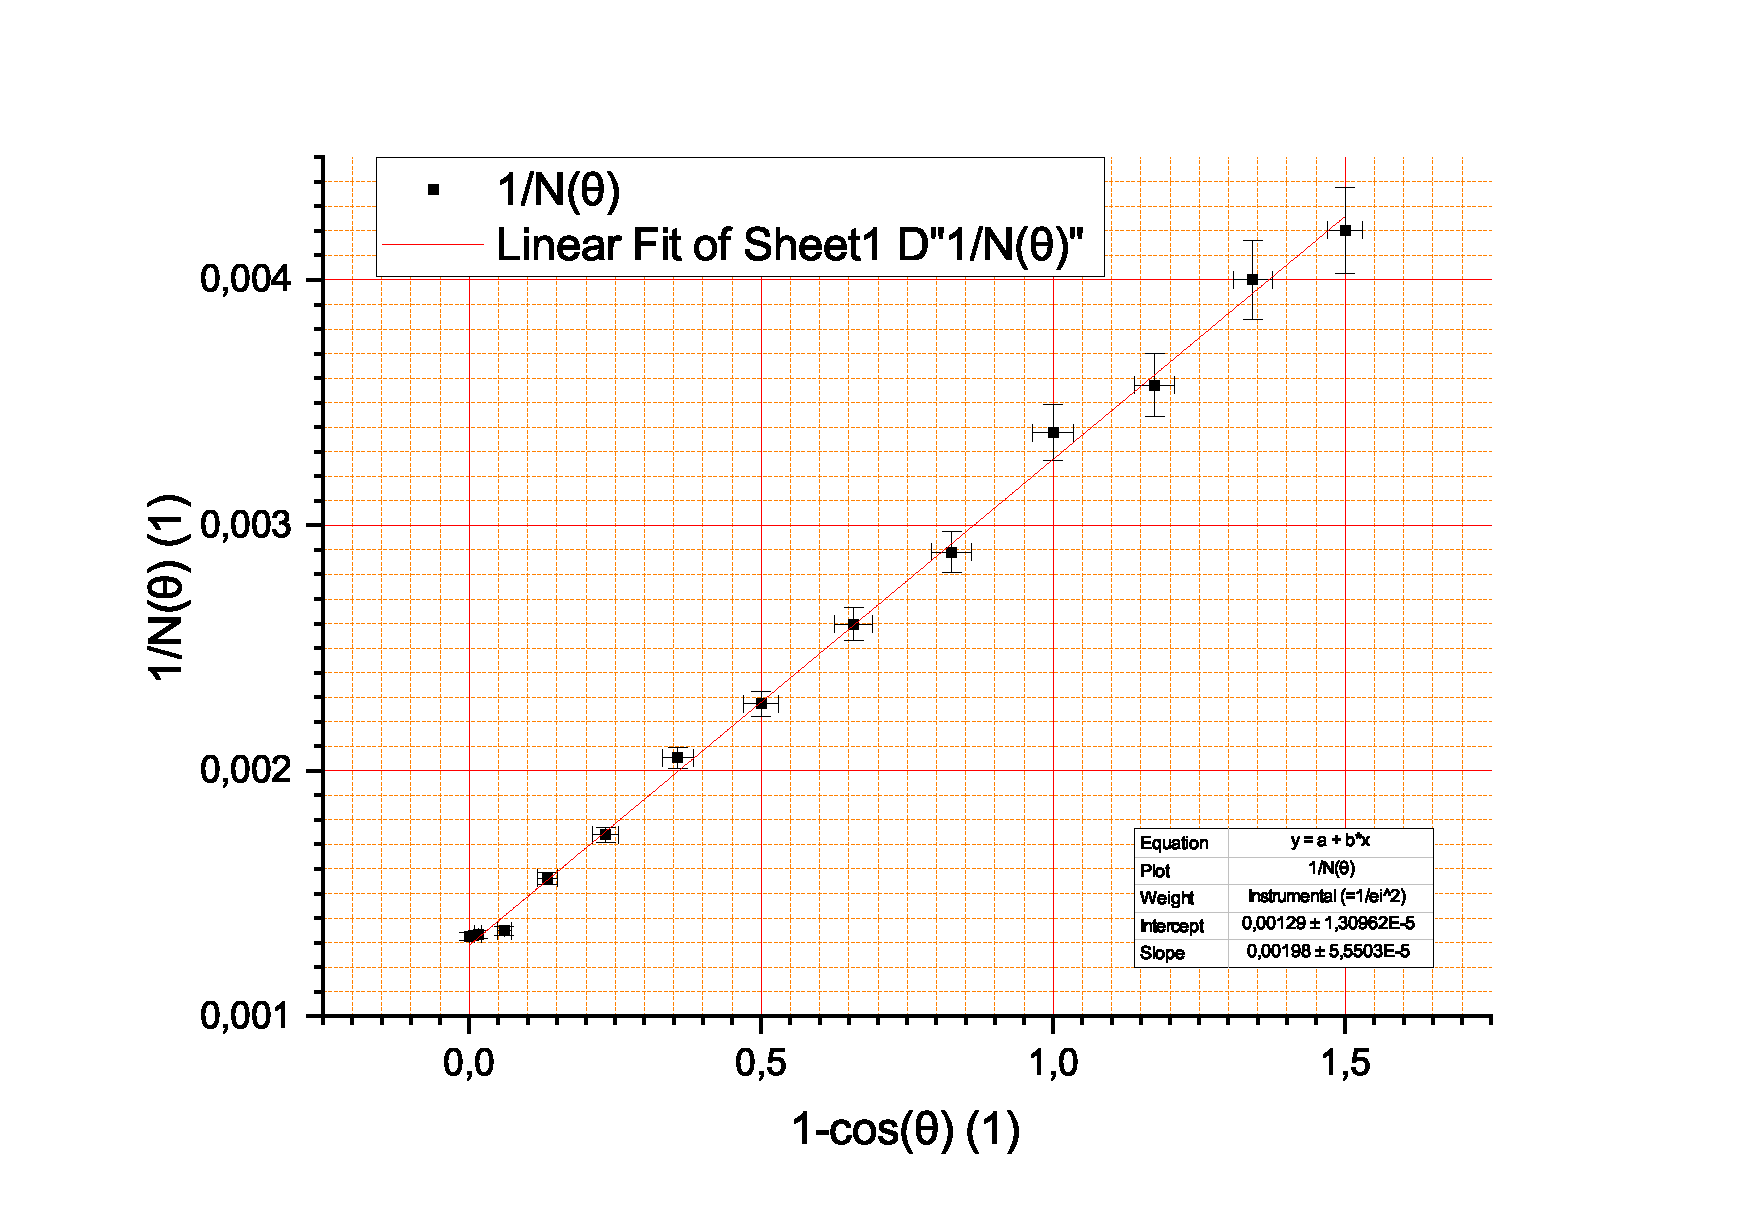
\includegraphics[width=\textwidth]{Graph1}
    \caption{Спектр источника излучения}
    \label{fig:vac}
\end{figure}

\item По графику, приведённому на рис. 5, определяем, что большая часть гамма-квантов с нужной нам энергией 23,8 кэВ появляется при пороговых значениях от 3 В до 7 В. Установим эти значения на выпрямителе. По окончании этого этапа электронная схема нашей установки настроена так, что
подсчитываются только гамма-кванты с энергиями, соответствующими используемому
источнику.
\end{enumerate}

\subsection{Измерение резонансного поглощения}
\begin{enumerate}
    \item Установим время измерения 20 секунд, ход поглотителя 8,84 мм.
    \item Измерим фоновое излучение. Вычитание фона в дальнейшем
производится компьютером автоматически. Измеренное значение фона: 10,5 1/сек.
    \item Проведём измерение спектра резонансного поглощения для трёх образцов: две оловянные пленки разной толщины и образец оксида олова SnO$_2$. Для этого проведём серию измерений при разных скоростях движения поглотителя. Результаты занесём в таблицы 2-4. 
    
    \begin{table}[h]
    \centering
    \begin{center}
    \caption{Поглотитель 1: Sn, толщина 90 мкм}
    \end{center}
    \vspace{0.1cm}
    \label{tab:my_label}
    \begin{tabular}{ |p{2.5cm}||p{1cm}|p{1cm}|p{1cm}|p{1cm}|p{1cm}|p{1cm}|p{1cm}|p{1cm}|p{1cm}|p{1cm}|p{1cm}|}
 \hline
 Скорость, мм/с & 0 & 0,87 & 1,28 & 1,3 & 1,53 & 1,7 & 1,92 & 1,92 & 2,02 & 2,12 & 2,34

 \\
\hline
 Интенсивность, счёт. & 1311,8 & 1258,2 & 1254,3 & 1232,5 & 1219,2 & 1222,9 & 1192,1 & 1179,4 & 1147 & 1129,8 & 1125,4

\\
\hline
\hline
Скорость, мм/с & 2,39 & 2,4 & 2,5 & 2,51 & 2,56 & 2,61 & 2,66 & 2,92 & 3,1 & 3,36 & 3,67

 \\
 \hline
 Интенсивность, счёт.  & 1122,7 & 1116,4 & 1123,8 & 1148,3 & 1145,9 & 1156,3 & 1154,3 & 1189,2 & 1212,2 & 1223,4 & 1251,4
\\
 \hline
\end{tabular}
\end{table} 

\begin{table}[h]
    \centering
    \begin{center}
    \caption{Поглотитель 2: Sn, толщина 180 мкм}
    \end{center}
    \vspace{0.1cm}
    \label{tab:my_label}
    \begin{tabular}{ |p{2.5cm}||p{1cm}|p{1cm}|p{1cm}|p{1cm}|p{1cm}|p{1cm}|p{1cm}|p{1cm}|p{1cm}|p{1cm}|p{1cm}|}
 \hline
 Скорость, мм/с & 0 & 0,7 & 1,32 & 1,59 & 1,6 & 1,65 & 1,66 & 1,66 & 1,68 & 1,68 & 1,69
 \\
\hline
 Интенсивность, счёт. & 587,8 & 599,1 & 581,2 & 579 & 572,9 & 573 & 587,8 & 577,8 & 564,3 & 551,2 & 567,2
\\
\hline
\hline
Скорость, мм/с & 1,71 & 1,87 & 1,92 & 2,05 & 2,08 & 2,2 & 2,29 & 2,34 & 2,39 & 2,44 & 2,47
 \\
 \hline
 Интенсивность, счёт.  & 552,5 & 550,4 & 538,8 & 528,4 & 514,2 & 508,8 & 497,4 & 485,6 & 497 & 511,8 & 499,4
\\
 \hline
 \hline
Скорость, мм/с & 2,57 & 2,62 & 3,35 & 3,47 & 3,58 & 3,65 & 3,75 & 5,28 & 6,06 & & 

 \\
 \hline
 Интенсивность, счёт.  & 515,6 & 521,8 & 524,4 & 532 & 561,1 & 545,8 & 563,8 & 552,2 & 560,9 & & 
\\
 \hline
\end{tabular}
\end{table}

\begin{table}[h]
    \centering
    \begin{center}
    \caption{Поглотитель 4: SnO$_2$}
    \end{center}
    \vspace{0.1cm}
    \label{tab:my_label}
    \begin{tabular}{ |p{2.5cm}||p{1cm}|p{1cm}|p{1cm}|p{1cm}|p{1cm}|p{1cm}|p{1cm}|p{1cm}|p{1cm}|p{1cm}|p{1cm}|}
 \hline
 Скорость, мм/с & -2,84 & -2,33 & -2,22 & -2,07 & -1,72 & -1,7 & -1,68 & -1,21 & -1,13 & -0,92 & -0,91
 \\
\hline
 Интенсивность, счёт. & 997,4 & 1003,4 & 995,2 & 979,2 & 968,2 & 973,3 & 967,7 & 893 & 874,2 & 815,6 & 831,3
\\
\hline
\hline
Скорость, мм/с & -0,88 & -0,86 & -0,59 & -0,56 & -0,28 & -0,13 & 0,16 & 0,3 & 0,57 & 0,58 & 0,85
\\
 \hline
 Интенсивность, счёт.  & 815,8 & 806 & 758,4 & 752,5 & 719 & 708,4 & 710,8 & 725 & 769,3 & 763,6 & 826,4
\\
 \hline
 \hline
Скорость, мм/с & 0,87 & 0,88 & 0,91 & 1,09 & 1,17 & 1,66 & 1,7 & 1,7 & 2,06 & 2,19 & 3,07
\\
 \hline
 Интенсивность, счёт.  & 837,2 & 836,5 & 840,5 & 883,7 & 890 & 939,7 & 956,8 & 956,8 & 977,3 & 1001,4 & 986,8
 \\
 \hline
\end{tabular}
\end{table}

\item По результатам измерения построим графики спектров резонансного поглощения для разных поглотителей (рис. 6-8). По графикам определим амплитуду резонансного поглощения в максимуме (в процентах), величину химического сдвига (в мм/с и в эВ) и экспериментальную ширину линии $\Gamma$. Результаты измерений занесём в таблицу 5. \par

Формула для вычисления величины амплитуды эффекта Мессбауэра:
\begin{equation}
    \varepsilon(v) = \frac{N(\infty) - N(v)}{N(\infty) - N_b},
\end{equation}
где $N(\infty)$ - скорость счёта квантов при достаточно большой скорости, $N(v)$ - скорость счёта квантов, прошедших через поглотитель при некоторой скорости, $N_b$ - скорость счёта радиоактивного фона (вычитается программой автоматически). \par
Величина химического сдвига, выраженная в эВ:
\begin{equation}
    \triangle E = E \frac{v}{c},
\end{equation}
где $E$ - энергия гамма-кванта, излучаемого веществом (в нашем случае $E = 23.8$ кэВ). \par
Экспериментальная ширина линии $\Gamma_e$, выраженная в эВ:
\begin{equation}
    \Gamma_e = 2 \Gamma = E \frac{v_{\Gamma}}{c},
\end{equation}


\begin{figure}[h]
    \centering
    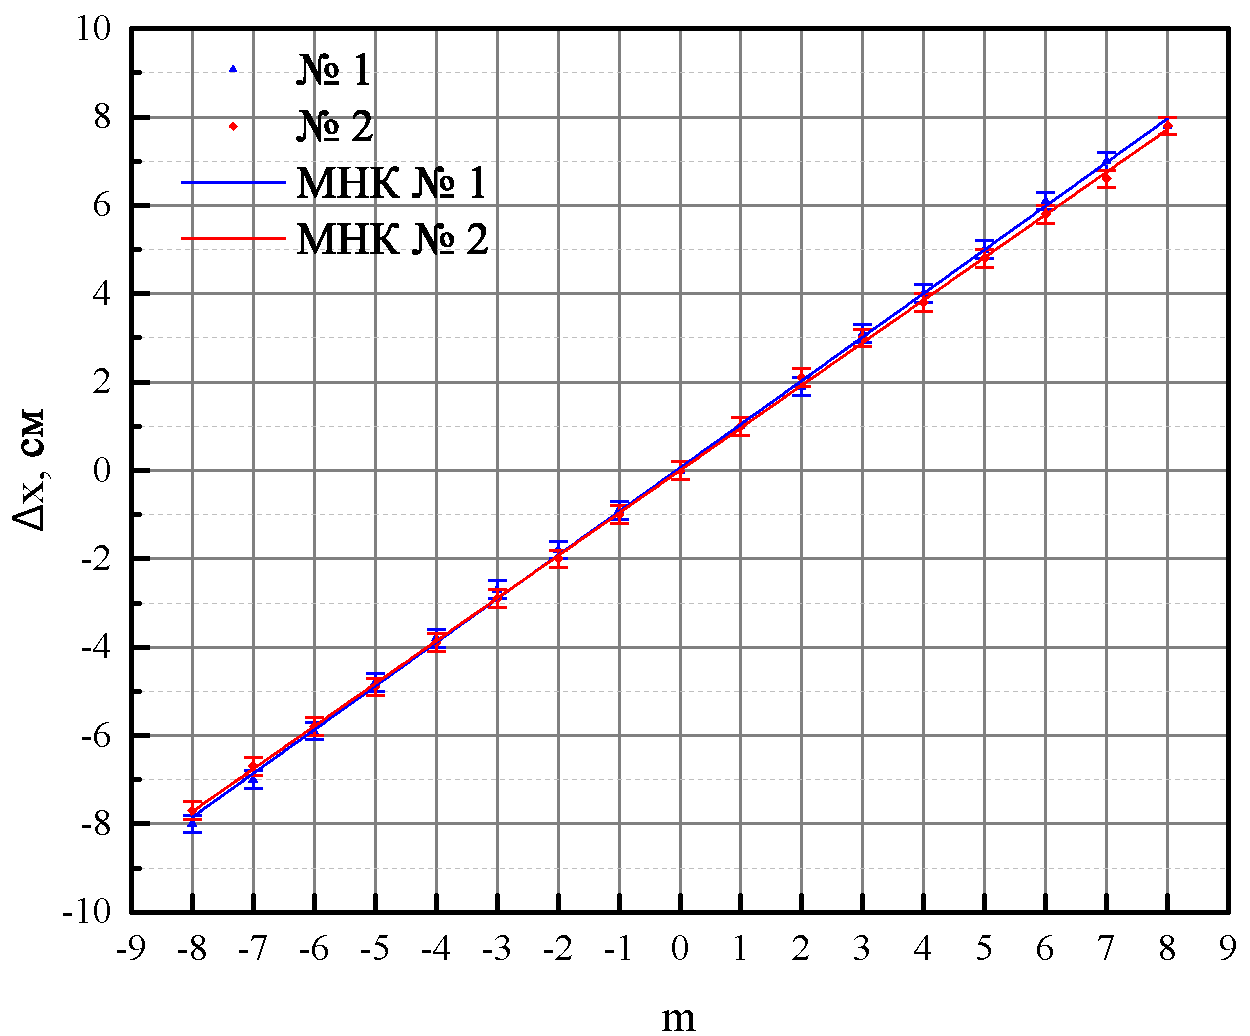
\includegraphics[width=12cm]{Graph2}
    \caption{Спектр резонансного поглощения: поглотитель 1}
    \label{fig:vac}
\end{figure}

\begin{figure}[h]
    \centering
    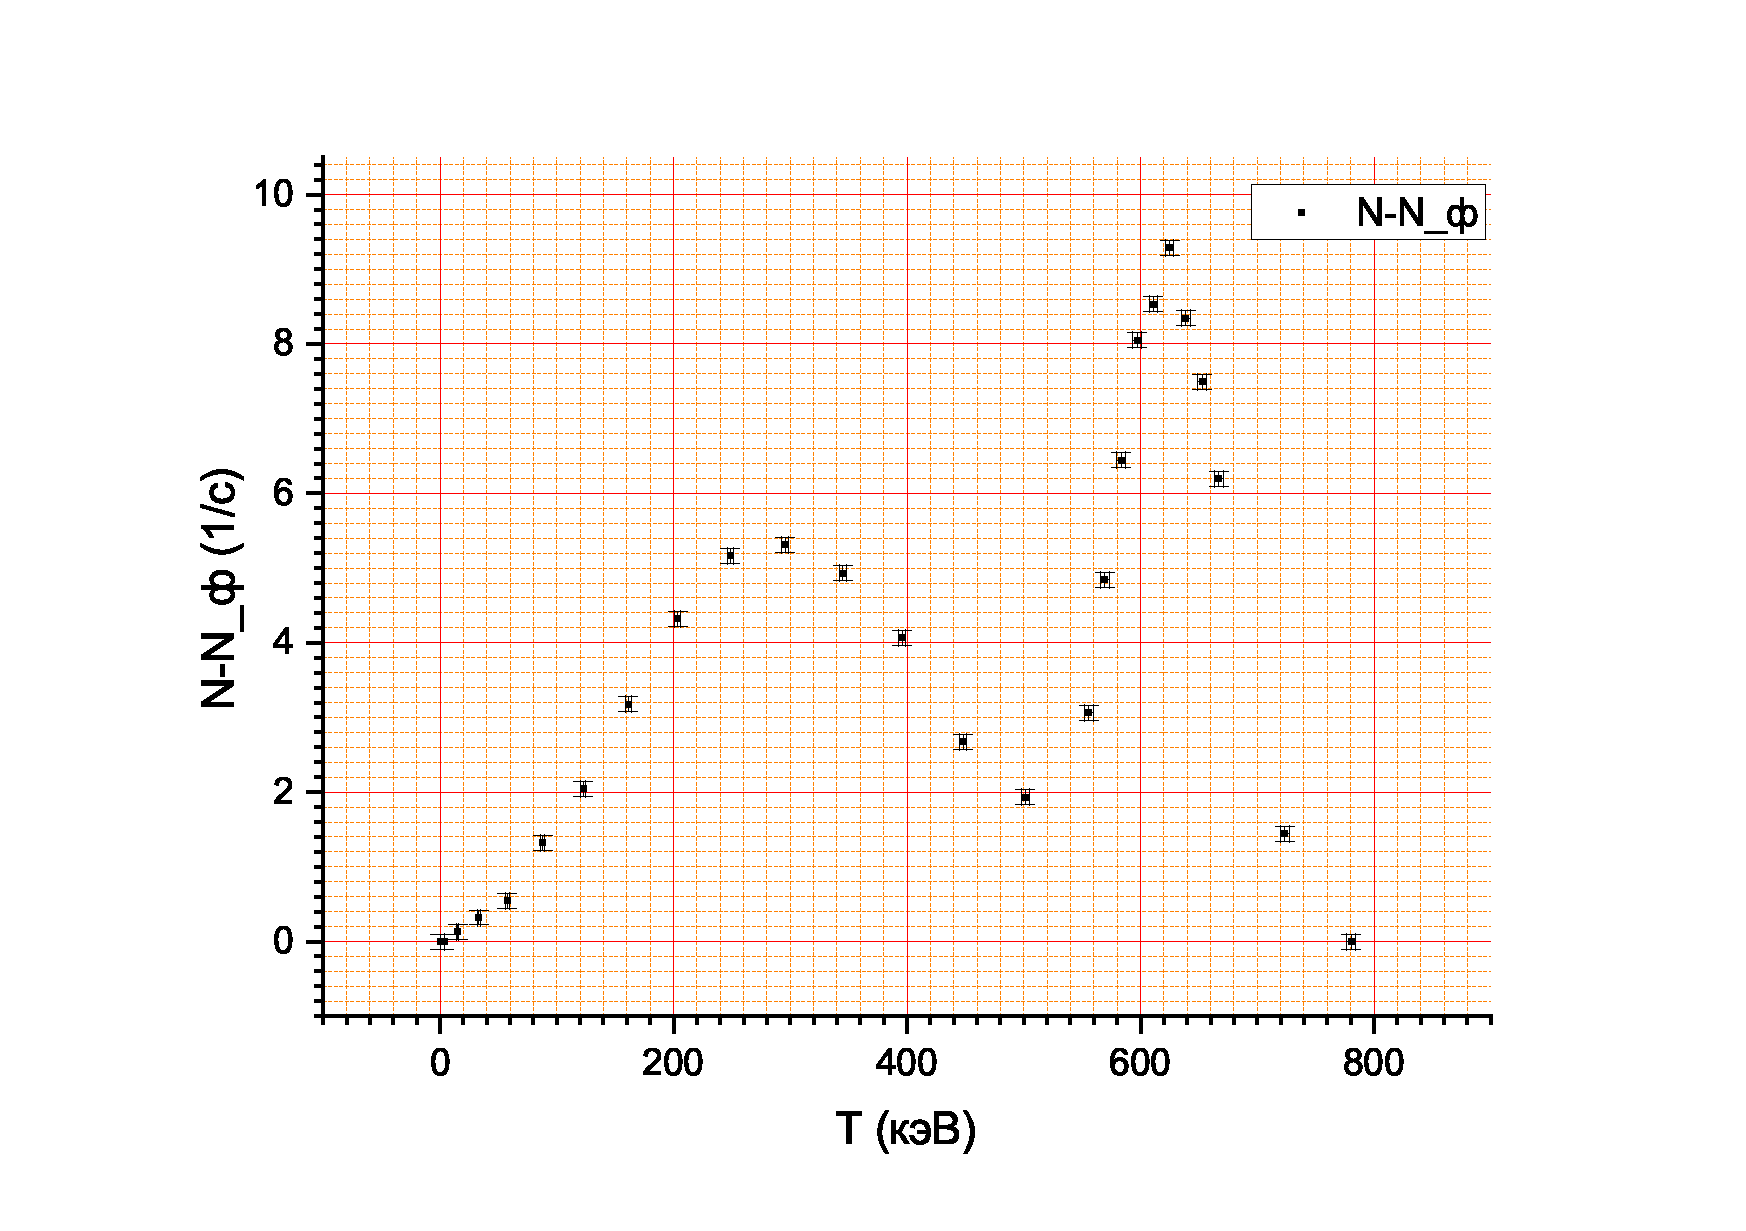
\includegraphics[width=12cm]{Graph3}
    \caption{Спектр резонансного поглощения: поглотитель 2}
    \label{fig:vac}
\end{figure}

\begin{figure}[h]
    \centering
    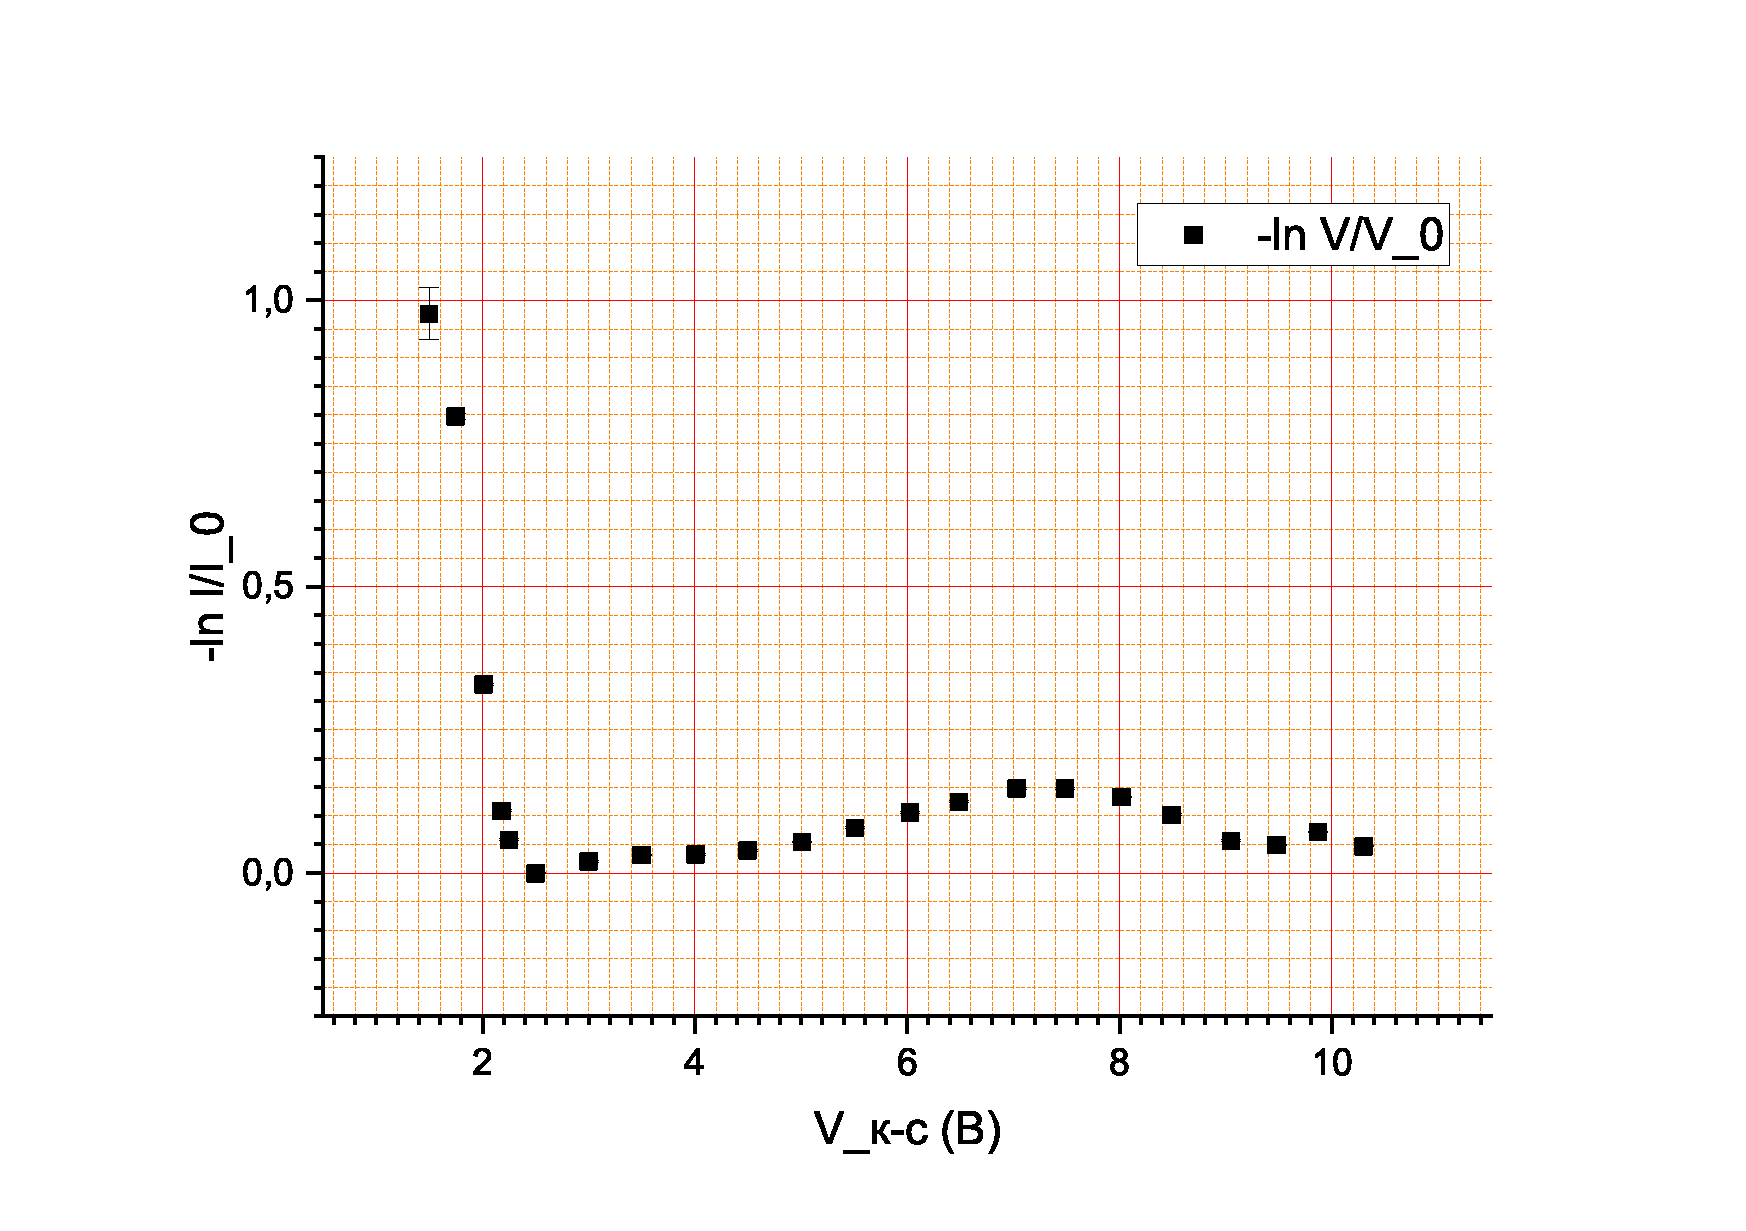
\includegraphics[width=12cm]{Graph4}
    \caption{Спектр резонансного поглощения: поглотитель 4}
    \label{fig:vac}
\end{figure}


\begin{table}[h]
    \centering
    \begin{center}
    \caption{Полученные значения}
    \end{center}
    \vspace{0.1cm}
    \label{tab:my_label}
    \begin{tabular}{ |p{3cm}||p{2cm}|p{2cm}|p{2cm}|p{2cm}|p{2cm}|}
\hline
    & Амплитуда эффекта, \% & Хим. сдвиг, мм/с & Хим. сдвиг, эВ & $\Gamma_e$, мм/с & $\Gamma_e$, эВ  \\
\hline
\hline
Поглотитель 1 & 11,3 & 2,4 & 1,90 $\cdot$ 10$^{-3}$ & 1 & 7,93 $\cdot$ 10$^{-3}$\\
\hline
Поглотитель 2 & 17,4 & 2,34 & 1,86 $\cdot$ 10$^{-3}$ & 1,55 & 12,30 $\cdot$ 10$^{-3}$\\
\hline
Поглотитель 4 & 29,4 & 0 & 0 & 2 & 15,90 $\cdot$ 10$^{-3}$\\
\hline
\end{tabular}
\end{table} 

\item Приведём на одном графике результаты измерения спектров резонансного поглощения для разных поглотителей (рис. 9). Видно, что увеличение толщины поглотителя уширяет резонансную линию (см. вывод)

\begin{figure}[h]
    \centering
    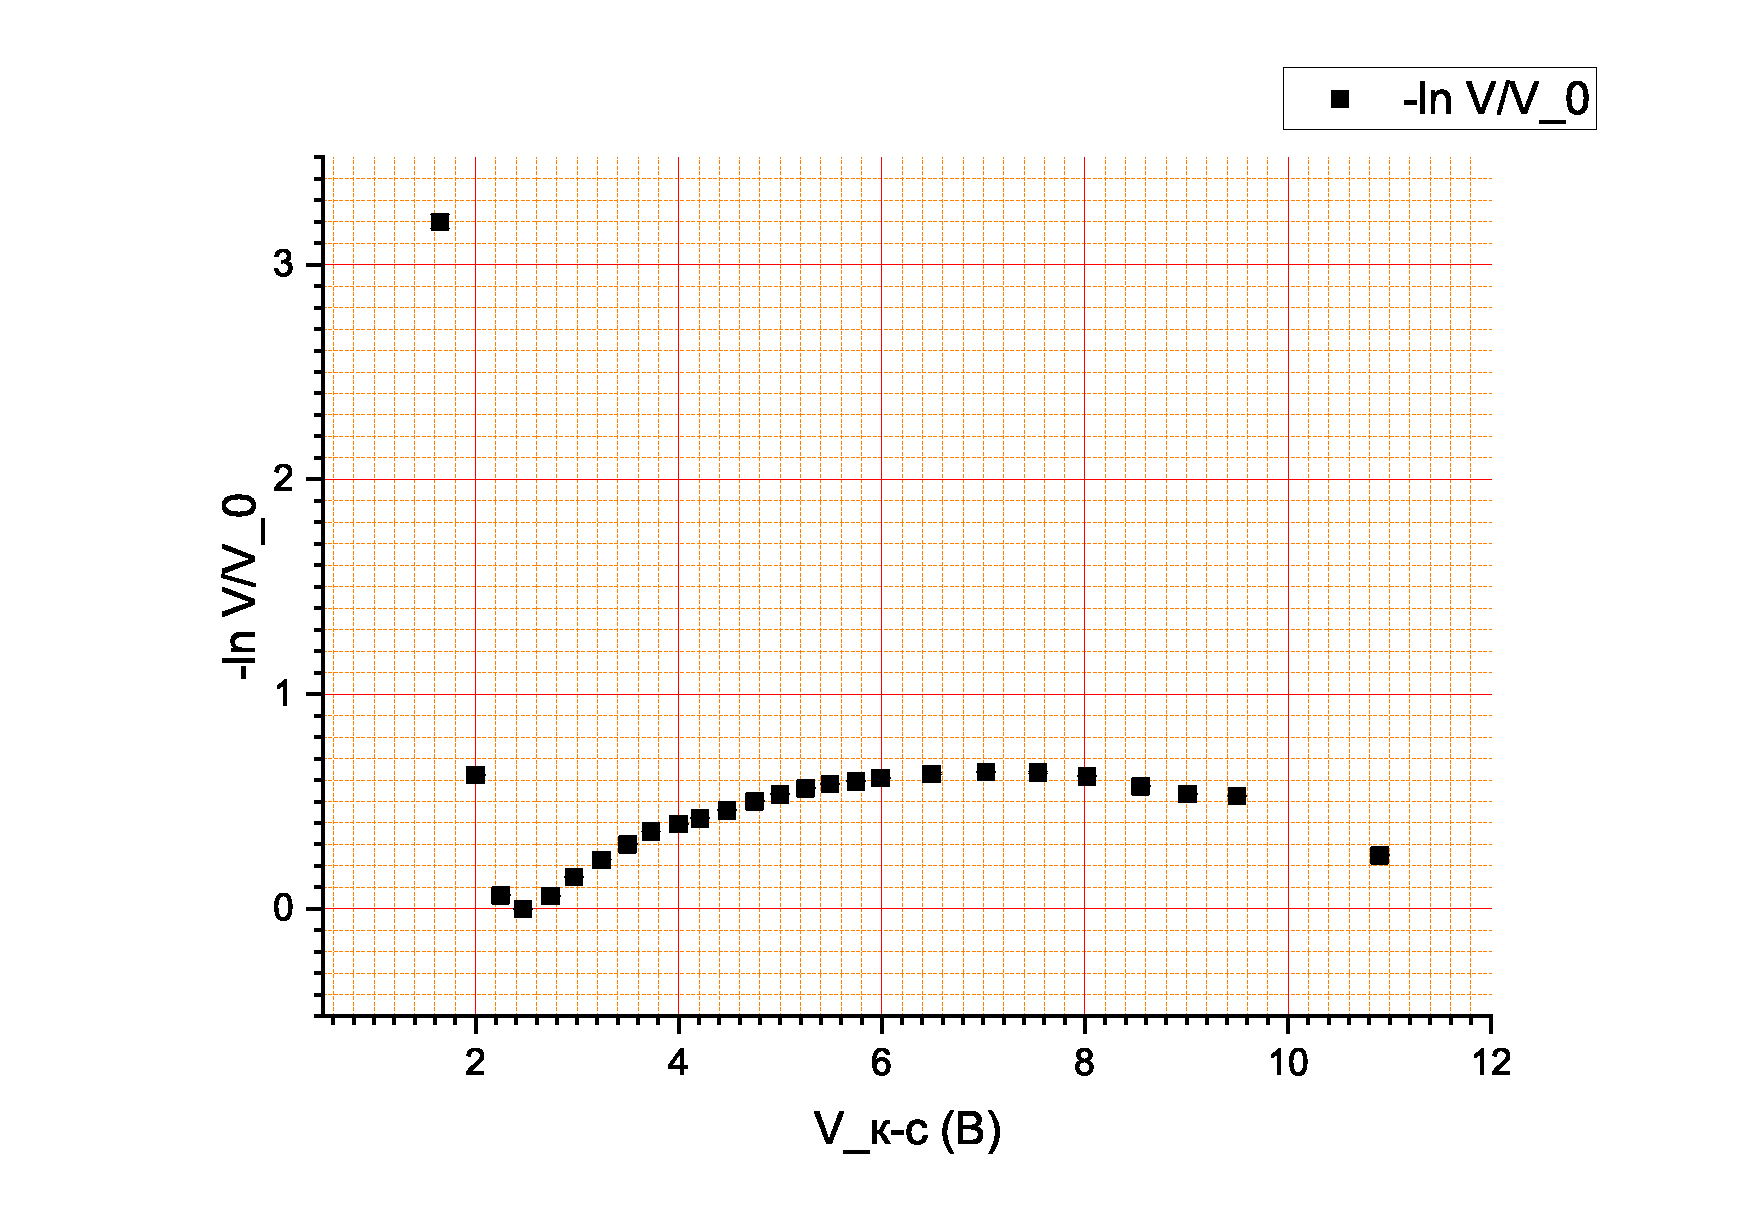
\includegraphics[width=15cm]{Graph5}
    \caption{Спектры резонансного поглощения: различные поглотители}
    \label{fig:vac}
\end{figure} \clearpage

\item Оценим время жизни возбуждённого состояния ядра Sn-119, используя формулу (3): $\Gamma \propto 10^{-7} eV$ в эксперименте; естественная ширина $\Gamma \propto 3 \cdot 10^{-8} eV$:
\begin{center}
    $\tau \simeq \frac{\hbar}{\Gamma}$ \\
    $\tau \simeq 0.7 \cdot 10^{-8} eV$ - по экспериментальным данным\\
    $\tau \simeq 2.1 \cdot 10^{-8} eV$  - по табличным данным без уширения\\
\end{center}

\end{enumerate}


\section{Вывод}
\begin{enumerate}
\item В ходе работы с помощью метода доплеровского сдвига для нескольких образцов поглотителя Sn были определены амплитуда резонансного поглощения, химический сдвиг и экспериментальное значение ширины спектральной линии - см. таблицу 5. Естественная ширина спектральной линии составляет $\Gamma = 3 \cdot 10^{-8} $эВ, что в несколько раз меньше значений, полученных экспериментально, но совпадает с ними по порядку величины. Это объясняется тем, что при комнатной температуре большую роль играет доплеровское уширение. 
\item Были исследованы графики спектров резонансного поглощения различных образцов (см. рис. 9). Наблюдаются следующие эффекты:
\begin{itemize}
    \item уширение резонансной линии при увеличении толщины слоя поглотителя. Возможные объяснения:
    \begin{itemize}
        \item кванты, энергия которых лежит вблизи максимума линии, сильно поглощаются уже в тонком поглотителе, и для них увеличение толщины поглотителя сказывается слабее, чем на "крыльях" линии
        \item самопоглощение квантов в источнике, если в нём содержатся резонансно поглощающие ядра
        \item доплеровское уширение как причина аппаратурного уширения, связанного с вибрациями источника и поглотителя
        \item неравномерность скорости перемещения поглотителя относительно источника
    \end{itemize}
    \item уменьшение регистрируемой интенсивности при увеличении толщины слоя поглотителя (больше гамма-квантов поглощаются на пути к ФЭУ)
    \item отсутствие химического сдвига у соединения оксида олова SnO$_2$
\end{itemize}
\item Было оценено время жизни мессбауэровского ядерного уровня 23,8 кэВ: по порядку величины оно совпало с табличным значением $\tau \simeq \cdot 10^{-8} eV$ (при полученных значениях $0.7 \cdot 10^{-8} eV$ и $2.1 \cdot 10^{-8} eV$ для естественной ширины линии и расчётной из эксперимента соответственно)
\end{enumerate}

\end{document}
